\appendix
\section{Reproducibility and Supporting Data}
\label{sec:appendix}
This appendix is the reference register for the active nominal scenario, not a second model derivation. K identifies authoritative published information, E a literature/readout estimate, and A a project assumption. E/A combines sourced information with a geometric, configuration or operating assumption. Computed outputs inherit the evidence limits of their inputs. SI units apply unless explicitly shown otherwise; angles in code are radians, while some input records and plots use degrees.

\subsection{Evidence and vehicle-input register}
\label{sec:appendix-evidence}
Table~\ref{tab:app-sources} resolves the source chain used by the register. The numeric vehicle definitions are in \path{vehicle_parameters.py}; \path{data/vehicle_parameters.json} supplies metadata rather than an independent set of numeric overrides. Cargo metadata resolves to the official CRS-10 overview. The executed rotating-frame, two-child and gyro-driven navigation paths are identified in the configuration and saved run; numeric inputs and explicit implementation choices take precedence over older prose descriptions.

\begingroup\small\setlength{\tabcolsep}{4pt}\renewcommand{\arraystretch}{1.1}
\begin{longtable}{@{}>{\raggedright\arraybackslash}p{0.23\linewidth}>{\raggedright\arraybackslash}p{0.21\linewidth}>{\raggedright\arraybackslash}p{0.15\linewidth}>{\raggedright\arraybackslash}p{0.35\linewidth}@{}}
\caption{Evidence sources and applicability.}\label{tab:app-sources}\\
\toprule
Input family & Source / locator & Status & Scope limitation \\
\midrule\endfirsthead
\multicolumn{4}{l}{\small\textit{Table \ref{tab:app-sources} continued}}\\
\toprule
Input family & Source / locator & Status & Scope limitation \\
\midrule\endhead
\midrule\multicolumn{4}{r}{\small\textit{Continued on next page}}\\\endfoot
\bottomrule\endlastfoot
Official mission schedule & \cite[PDF p.~2]{nasacrs10press} & K publication; A commands & Approximate preflight times; not measured thresholds or restart states. \\
Cargo inventory & \cite{nasacrs10overview} & K & $1530+960=2490\,\mathrm{kg}$; already inside loaded Dragon mass. \\
External vehicle geometry & \cite[Table 2-1]{spacexguide2025} & K / E/A use & Later guide; exterior diameter, not 2017 internal dimensions. \\
Legacy stage lengths & \cite{faa2018} & E/A & FT fact sheet plus assumed contiguous stage datums. \\
Mass/engine research set & \cite[Tables 2.16--2.18]{pezent2024} & E & Printed p.77 / PDF p.94; not a mission-certified operating set. \\
Effective sea-level point & \cite[Sec.2.2, p.11]{spacex2015} & E/A use & Historical 756 kN reference combined with the adopted nozzle model. \\
Structural tank envelope & \cite[Table 1]{ecker2017} & E/A & Reverse-engineered structural dimensions, mapped to flat liquid columns. \\
Dry groups / consumed O/F & \cite[Table 2 / Sec.2.2]{bykerk2023} & E/A / E & Generic research vehicle; group shapes and residual placement assumed. \\
Initial tank inventories & \cite[Table 1, p.215]{romerocalco2023} & E & Only published capacities adopted; no in-flight inventory measurement. \\
Liquid reference properties & \cite[Table 5, PDF p.24]{miquel2020} & E & Comparative reference temperatures/densities; pressure unspecified. \\
Loaded Dragon mass & \cite{kyledatasheet} & E, provisional & External approximate 8430 kg estimate; original host may be inaccessible; no official mass confirmation. \\
Dragon envelope & \cite[p.26 / PDF p.27]{crs1presskit} & E/A & Earlier Dragon 1 capsule/trunk dimensions, transferred to a uniform equivalent. \\
Ascent readout & \cite{crs10webcast,crs10telemetry} & E & Author-published digitization of broadcast readouts; calibration and comparison share the record. \\
Atmospheric layers & \cite{ussa1976} & K model / A use & Published standard profile, not measured CRS-10 weather. \\
\end{longtable}\endgroup

Table~\ref{tab:app-vehicle} consolidates the independent vehicle inputs and selected derived checks. All stations are from the original stack base along $+x_B$ unless stated as local. No fairing mass or extra cargo mass is added. Engine masses close the stage dry budgets; they are not added a second time.

\begingroup\small\setlength{\tabcolsep}{4pt}\renewcommand{\arraystretch}{1.1}
\begin{longtable}{@{}>{\raggedright\arraybackslash}p{0.29\linewidth}>{\raggedright\arraybackslash}p{0.25\linewidth}>{\raggedright\arraybackslash}p{0.06\linewidth}>{\raggedright\arraybackslash}p{0.34\linewidth}@{}}
\caption{Vehicle and engine input register; paired entries follow the order named.}\label{tab:app-vehicle}\\
\toprule
Parameter & Adopted value & Class & Basis / implementation meaning \\
\midrule\endfirsthead
\multicolumn{4}{l}{\small\textit{Table \ref{tab:app-vehicle} continued}}\\
\toprule
Parameter & Adopted value & Class & Basis / implementation meaning \\
\midrule\endhead
\midrule\multicolumn{4}{r}{\small\textit{Continued on next page}}\\\endfoot
\bottomrule\endlastfoot
Outer diameter / radius & $3.66/1.83\,\mathrm{m}$ & K & \cite[Table 2-1]{spacexguide2025}; radius derived. \\
Stage-1 / stage-2 lengths & $42.6/12.6\,\mathrm{m}$ & E/A & \cite{faa2018}; assumed attachment boundary. \\
Stage-1 dry / initial propellant & $22200/410900\,\mathrm{kg}$ & E & \cite[Table 2.17]{pezent2024}. \\
Stage-2 dry / initial propellant & $4000/107500\,\mathrm{kg}$ & E & \cite[Table 2.17]{pezent2024}. \\
Loaded Dragon / included cargo & $8430/2490\,\mathrm{kg}$ & E / K & \cite{kyledatasheet,nasacrs10overview}; cargo is a subset. \\
Dragon length / radius & $7.2/1.83\,\mathrm{m}$ & E/A & \cite{crs1presskit}; $4.4+2.8$ m envelope, uniform solid cylinder. \\
Stage-2 local / stack CG & $6.3/48.9\,\mathrm{m}$ & A & Equivalent uniform midpoint plus 42.6 m offset. \\
Dragon stack CG & $58.8\,\mathrm{m}$ & A & $42.6+12.6+7.2/2$; not measured. \\
Total mass / model height & $553030\,\mathrm{kg}$ / $62.4\,\mathrm{m}$ & E/A & Sums of the adopted masses and axial envelopes. \\
RP-1 / LOX loading & $123500/287400\,\mathrm{kg}$ & E & \cite[Table 1]{romerocalco2023}. \\
Loaded / consumed O/F & $2.3271255/2.35$ & E & Inventory ratio / \cite[Sec.2.2]{bykerk2023}. \\
RP-1 / LOX skin thickness & $0.0031/0.0029\,\mathrm{m}$ & E & \cite[Table 1]{ecker2017}; modeled skins. \\
RP-1 / LOX inner radius & $1.8269/1.8271\,\mathrm{m}$ & E/A & Outer radius minus the adopted skin; no hardware displacement. \\
RP-1 / LOX bottom station & $4.0/18.7\,\mathrm{m}$ & E/A & \cite[Table 1]{ecker2017}; aligned flat bottoms. \\
RP-1 / LOX tank length & $14.7/22.1\,\mathrm{m}$ & E/A & \cite[Table 1]{ecker2017}; structural envelopes. \\
RP-1 density / temperature & $820\,\mathrm{kg\,m^{-3}}$ / $266\,\mathrm{K}$ & E & \cite[Table 5]{miquel2020}; constant reference property. \\
LOX density / temperature & $1250\,\mathrm{kg\,m^{-3}}$ / $66\,\mathrm{K}$ & E & \cite[Table 5]{miquel2020}; pressure unspecified. \\
Dry shell: mass / CG / length & $8000\,\mathrm{kg}$ / $21/42\,\mathrm{m}$ & E/A & \cite[Table 2]{bykerk2023}; thin-shell equivalent. \\
Dry fins: mass / CG & $1520\,\mathrm{kg}$ / $40.3\,\mathrm{m}$ & E/A & \cite[Table 2]{bykerk2023}; equivalent disk. \\
Dry engines: mass / CG & $4230\,\mathrm{kg}$ / $0.452\,\mathrm{m}$ & E/A & \cite[Table 2]{bykerk2023}; equivalent disk. \\
Folded legs: mass / CG & $2000\,\mathrm{kg}$ / $6.66\,\mathrm{m}$ & E/A & \cite[Table 2]{bykerk2023}; fixed mass placement. \\
Residual dry mass / interval & $6450\,\mathrm{kg}$ / $[4,40.8]\,\mathrm{m}$ & A & Budget closure; uniform thin-shell equivalent, centroid 22.4 m. \\
Nominal dry CG & $17.52108\,\mathrm{m}$ & E/A & Mass-weighted adopted dry allocation. \\
Dry inertia, axial / transverse & $61368.59$ / $4441994.04\,\mathrm{kg\,m^2}$ & E/A & Computed component equivalents; not measured inertia. \\
Stage-1 / stage-2 engine count & $9/1$ & K & Falcon configuration \cite{spacex2015}; modeled as central + ring / MVac. \\
Vacuum thrust, stage 1 / 2 & $824901/935000\,\mathrm{N}$ & E/A; E & 756000 + $0.68(101325)$ / \cite[Table 2.16]{pezent2024}. \\
Vacuum $I_{\mathrm{sp}}$, stage 1 / 2 & $311/348\,\mathrm{s}$ & E & \cite[Table 2.16]{pezent2024}. \\
Exit area, stage 1 / 2 & $0.68/4.90\,\mathrm{m^2}$ & E & \cite[Table 2.16]{pezent2024}. \\
Minimum steady throttle, 1 / 2 & $0.60/0.40$ & E & \cite[Table 2.16]{pezent2024}; off is separate. \\
Reference pressure / $g_0$ & $101325\,\mathrm{Pa}$ / $9.80665\,\mathrm{m\,s^{-2}}$ & K & Standard reference constants \cite{ussa1976}. \\
Stage-1 sea-level thrust / $I_{\mathrm{sp}}$ & $756000\,\mathrm{N}$ / $285.023\,\mathrm{s}$ & E/A & Derived at the reference pressure and retained flow. \\
Engine dry proxy, stage 1 / 2 & $470/700\,\mathrm{kg}$ & E & \cite[Table 2]{bykerk2023}; inside stage budgets. \\
Engine ring / pivot, stage 1 & $1.3/1.0\,\mathrm{m}$ & A & Ring radius / axial force pivot; not engine CG. \\
Stage-2 local pivot & $0.5\,\mathrm{m}$ & A & From its own base. \\
Stored gimbal limits, stages 1/2 & $5^\circ/5^\circ$ & A & Stored input only; physical gimbal dynamics are inactive. \\
\end{longtable}\endgroup

The stage-1 liquid model is \texttt{dual\_tank}; stage 2 uses an equivalent uniform propellant cylinder. Inventory reconstruction assumes fixed O/F, no venting/refilling, fixed initial loading, constant density, and settled flat columns. Dry and payload shape equivalents, no slosh, balanced fixed exhaust ports and unchanged folded-leg mass placement are A-class closures. The $1202.128\,\mathrm{kg}$ limiting RP-1 residual is a consequence of the adopted loading/consumption pair, not the separately protected $2000\,\mathrm{kg}$ mission reserve.

\subsection{Environment and aerodynamic register}
Table~\ref{tab:app-environment} lists environmental constants and all atmosphere/wind knots. Layer bases use the code's radial-altitude coordinate; the standard profile is a reference atmosphere rather than measured launch weather.

\begingroup\small\setlength{\tabcolsep}{4pt}\renewcommand{\arraystretch}{1.1}
\begin{longtable}{@{}>{\raggedright\arraybackslash}p{0.29\linewidth}>{\raggedright\arraybackslash}p{0.25\linewidth}>{\raggedright\arraybackslash}p{0.06\linewidth}>{\raggedright\arraybackslash}p{0.34\linewidth}@{}}
\caption{Active environment inputs and optional wind-profile definition.}\label{tab:app-environment}\\
\toprule
Parameter & Value / knots & Class & Basis / limitation \\
\midrule\endfirsthead
\multicolumn{4}{l}{\small\textit{Table \ref{tab:app-environment} continued}}\\
\toprule
Parameter & Value / knots & Class & Basis / limitation \\
\midrule\endhead
\midrule\multicolumn{4}{r}{\small\textit{Continued on next page}}\\\endfoot
\bottomrule\endlastfoot
Earth / ground sphere & $R_E=6371000\,\mathrm{m}$; ground offset $0\,\mathrm{m}$ & A & Spherical Earth approximation; \path{Environement.py}. \\
Gravity normalization & $g_0=9.80665\,\mathrm{m\,s^{-2}}$; $\mu=g_0R_E^2$ & A & Central field normalized to the chosen surface value. \\
Earth rate / launch latitude & $7.292115\times10^{-5}\,\mathrm{rad\,s^{-1}}$ / $28.6^\circ$ & K / A & Sidereal-rate constant and rounded scenario latitude; launch-aligned axes. \\
Air gas constant / heat ratio & $287.05287\,\mathrm{J\,kg^{-1}\,K^{-1}}$ / $1.4$ & K & USSA reference constants \cite{ussa1976}. \\
Sea-level temperature / pressure & $288.15\,\mathrm{K}$ / $101325\,\mathrm{Pa}$ & K & USSA standard model \cite{ussa1976}. \\
Layer bases: $(h_b,T_b,L)$ & $(0,288.15,-0.0065)$; $(11000,216.65,0)$; $(20000,216.65,0.001)$ & K & $h_b$ [m], $T_b$ [K], $L$ [$\mathrm{K\,m^{-1}}$]; \cite{ussa1976}. \\
Remaining layer bases & $(32000,228.65,0.0028)$; $(47000,270.65,0)$; $(51000,270.65,-0.0028)$; $(71000,214.65,-0.002)$ & K & Same units and source. \\
Mesopause / model ceiling & $84852/2000000\,\mathrm{m}$ & K / A & Standard-layer endpoint / assumed numerical-vacuum-tail envelope. \\
Nominal surface wind / rotation & $[0,0,0]^{\mathsf T}\,\mathrm{m\,s^{-1}}$ / $0\,\mathrm{rad}$ & A & Default calm case; the entire scaled profile remains zero. \\
Wind knots $(h,	ext{scale})$ & $(0,1)$; $(100,1.2)$; $(1000,1.45)$; $(5000,1.75)$; $(11000,2)$ & A & Linear interpolation; altitude in m; stylized surface-reference multiplier. \\
Remaining wind knots & $(20000,1.1)$; $(32000,0.5)$; $(47000,0.15)$; $(71000,0.02)$; $(84852,0)$ & A & Exactly zero at and above 84852 m; no gusts/directional shear. \\
\end{longtable}\endgroup

Table~\ref{tab:app-aero-config} gives every declared configuration. Four serve the stack/booster sequence; the declared \texttt{second\_stack} is inactive in the upper-stage continuation, which instead uses $C_D=0.3$. $C_{N\alpha}$ is per radian; damping coefficients are dimensionless. Geometry is an equivalent envelope, and all normal-force, damping, fin and booster coefficients are A-class estimates. Only the original full-stack axial readout is E-class; applying its fairing geometry to Dragon remains A-class transfer.

\begingroup\small\setlength{\tabcolsep}{4pt}\renewcommand{\arraystretch}{1.1}
\begin{longtable}{@{}>{\raggedright\arraybackslash}p{0.2\linewidth}>{\raggedright\arraybackslash}p{0.2\linewidth}>{\raggedright\arraybackslash}p{0.16\linewidth}>{\raggedright\arraybackslash}p{0.38\linewidth}@{}}
\caption{Aerodynamic geometry, derivatives and projected side segments from the configuration JSON.}\label{tab:app-aero-config}\\
\toprule
Configuration & $S_{\mathrm{ref}}/L_{\mathrm{ref}}/x_p$ [$\mathrm{m^2}$/m/m] & $C_{N\alpha}/c_m/c_l$ & Segments: (bottom m, top m, width m, crossflow coefficient) \\
\midrule\endfirsthead
\multicolumn{4}{l}{\small\textit{Table \ref{tab:app-aero-config} continued}}\\
\toprule
Configuration & $S_{\mathrm{ref}}/L_{\mathrm{ref}}/x_p$ [$\mathrm{m^2}$/m/m] & $C_{N\alpha}/c_m/c_l$ & Segments: (bottom m, top m, width m, crossflow coefficient) \\
\midrule\endhead
\midrule\multicolumn{4}{r}{\small\textit{Continued on next page}}\\\endfoot
\bottomrule\endlastfoot
\path{full_stack} & $21.08/62.4/57.6$ & $2/-10/0$ & (0, 55.2, 3.66, 1.1); (55.2, 62.4, 3.7, 1.1) \\
\path{booster_alone} & $10.52/42.6/41$ & $2/-20/0$ & (0, 42.6, 3.66, 1.1) \\
\path{booster_return} & $10.52/42.6/41$ & $2/-20/-3$ & (0, 42.6, 3.66, 1.1); (38.6, 40.6, 2.4, 1) \\
\path{booster_landing} & $10.52/42.6/41$ & $2/-20/-3$ & (0, 42.6, 3.66, 1.1); (38.6, 40.6, 2.4, 1); (0, 3.6, 1.6, 1.2) \\
\path{second_stack} & $10.52/19.8/17.3$ & $2/-10/0$ & (0, 12.6, 3.66, 1.1); (12.6, 19.8, 3.7, 1.1) \\
\end{longtable}\endgroup

The common grid-fin control definition in \texttt{booster\_return} and \texttt{booster\_landing} has four fins at azimuths $45^\circ$, $135^\circ$, $225^\circ$, $315^\circ$ (stored rounded radian values), $1.65\,\mathrm{m^2}$ area per fin, slope $1.2\,\mathrm{rad^{-1}}$, pivot radius $1.83\,\mathrm{m}$, station $39.6\,\mathrm{m}$ and maximum deflection $0.35\,\mathrm{rad}$. These are A-class estimates, not measured fin effectiveness or actuator limits. The return and landing axial curves are identical; the deployed-leg side segment distinguishes their passive side-force geometry.

Table~\ref{tab:app-aero-knots} preserves the complete axial coefficient knots without interpolated values. A dash means that configuration has no original knot at that Mach value; the evaluator interpolates its own grid. The full-stack values through Mach 7 are digitized from Pezent's Figure~2.13(b) \cite{pezent2024}; Mach 8/10 extensions and the three other curves are A-class. Coefficients must retain their stated reference areas. Shape transfer to the CRS-10 loaded-Dragon envelope is unvalidated.

\begingroup\small\setlength{\tabcolsep}{4pt}\renewcommand{\arraystretch}{1.1}
\begin{longtable}{@{}>{\raggedright\arraybackslash}p{0.1\linewidth}>{\raggedright\arraybackslash}p{0.19\linewidth}>{\raggedright\arraybackslash}p{0.19\linewidth}>{\raggedright\arraybackslash}p{0.21\linewidth}>{\raggedright\arraybackslash}p{0.23\linewidth}@{}}
\caption{Complete stored zero-angle axial coefficient knots; return and landing share one column.}\label{tab:app-aero-knots}\\
\toprule
Mach & Full stack & Booster alone & Return / landing & Declared upper (inactive) \\
\midrule\endfirsthead
\multicolumn{5}{l}{\small\textit{Table \ref{tab:app-aero-knots} continued}}\\
\toprule
Mach & Full stack & Booster alone & Return / landing & Declared upper (inactive) \\
\midrule\endhead
\midrule\multicolumn{5}{r}{\small\textit{Continued on next page}}\\\endfoot
\bottomrule\endlastfoot
$0$ & $0.1416$ & $0.42$ & $0.67$ & $0.32$ \\
$0.05$ & $0.1289$ & --- & --- & --- \\
$0.1$ & $0.1221$ & --- & --- & --- \\
$0.2$ & $0.1173$ & --- & --- & --- \\
$0.4$ & $0.1124$ & --- & --- & --- \\
$0.6$ & $0.11$ & --- & --- & --- \\
$0.8$ & $0.1075$ & $0.41$ & $0.66$ & $0.31$ \\
$0.85$ & --- & $0.4$ & $0.65$ & $0.3$ \\
$0.9$ & $0.1075$ & --- & --- & --- \\
$0.92$ & $0.1552$ & --- & --- & --- \\
$0.94$ & $0.2631$ & --- & --- & --- \\
$0.96$ & $0.4257$ & --- & --- & --- \\
$0.98$ & $0.5954$ & --- & --- & --- \\
$1$ & $0.7655$ & $0.72$ & $0.97$ & $0.62$ \\
$1.02$ & $0.9342$ & --- & --- & --- \\
$1.04$ & $1.0799$ & --- & --- & --- \\
$1.05$ & --- & $0.94$ & $1.19$ & $0.84$ \\
$1.06$ & $1.1615$ & --- & --- & --- \\
$1.1$ & $1.1562$ & $0.92$ & $1.17$ & $0.82$ \\
$1.2$ & $1.1262$ & --- & --- & --- \\
$1.3$ & --- & $0.84$ & $1.09$ & $0.74$ \\
$1.4$ & $1.0732$ & --- & --- & --- \\
$1.6$ & $1.032$ & $0.74$ & $0.99$ & $0.66$ \\
$2$ & $0.9739$ & $0.68$ & $0.93$ & $0.6$ \\
$2.5$ & $0.9299$ & --- & --- & --- \\
$3$ & $0.9007$ & $0.56$ & $0.81$ & $0.48$ \\
$4$ & $0.8634$ & $0.5$ & $0.75$ & $0.42$ \\
$5$ & $0.8423$ & $0.46$ & $0.71$ & $0.38$ \\
$6$ & $0.8253$ & --- & --- & --- \\
$7$ & $0.8131$ & $0.42$ & $0.67$ & $0.36$ \\
$8$ & $0.79$ & $0.41$ & $0.65$ & $0.35$ \\
$10$ & $0.75$ & $0.4$ & $0.63$ & $0.34$ \\
\end{longtable}\endgroup

\subsection{Mission, control, sensor and filter settings}
\label{sec:appendix-settings}
All settings in Tables~\ref{tab:app-mission} and~\ref{tab:app-sensor-filter} are A-class scenario choices unless the table explicitly identifies a published timing anchor. They describe the executed full case after \path{recovery_plan} transforms clock-based entry/landing references into state-triggered conditions. The JSON's preflight entry/landing times are comparison markers, not the active restart clock.

\begingroup\small\setlength{\tabcolsep}{4pt}\renewcommand{\arraystretch}{1.1}
\begin{longtable}{@{}>{\raggedright\arraybackslash}p{0.23\linewidth}>{\raggedright\arraybackslash}p{0.4\linewidth}>{\raggedright\arraybackslash}p{0.33\linewidth}@{}}
\caption{Complete nominal mission/control setting groups and numerical criteria.}\label{tab:app-mission}\\
\toprule
Setting family & Value / active condition & Meaning / limitation \\
\midrule\endfirsthead
\multicolumn{3}{l}{\small\textit{Table \ref{tab:app-mission} continued}}\\
\toprule
Setting family & Value / active condition & Meaning / limitation \\
\midrule\endhead
\midrule\multicolumn{3}{r}{\small\textit{Continued on next page}}\\\endfoot
\bottomrule\endlastfoot
Initial structural base & $\vect r_O^B=[6371000,0,0]^{\mathsf T}\,\mathrm{m}$; $\vect v_O^B=\vect0$; $\vect\omega^B=\vect0$ & Base initially stationary relative to Earth. CG velocity includes migration. \\
Initial attitude / engines & $\vect q_{BE}=[\sqrt{1/2},0,-\sqrt{1/2},0]^{\mathsf T}$; nine engines at throttle 1 & Hamilton scalar-first; Body +x up. \\
Ascent pitch / PD gains & Start $8\,\mathrm{s}$; $\tau=100\,\mathrm{s}$; tilt cap $80^\circ$; $k_p=2\,\mathrm{s^{-2}}$, $k_d=2.5\,\mathrm{s^{-1}}$ & Unlimited ideal ascent couple. Stored heading $45^\circ$ is ignored by the active eastward target construction. \\
Shutdown / separation & Ramp $140$--$141\,\mathrm{s}$; separation $144\,\mathrm{s}$; zero flow/flow derivative and engines off & Published approximate anchors \cite{nasacrs10press}; one-second quintic envelope and no-impulse map assumed. \\
Return timing / engines & Guidance $0.2\,\mathrm{s}$; ramps $1\,\mathrm{s}$; boostback/entry indices $(0,1,5)$; landing $(0)$ & Allowed landing guidance interval is 0.01--0.2 s. \\
Fuel allocations / protected reserve & Boostback $38000$; entry $16000$; landing $10000$; reserve $2000\,\mathrm{kg}$ & Unused boostback/entry allocation can transfer; limiting-tank residual protected separately. \\
Boostback start / end design & $161\,\mathrm{s}$; throttle 1; window 10--60 s; predicted miss target $500\,\mathrm{m}$ & Fuel/duration cap can terminate before miss target. 500 kg anticipatory shutdown margin. \\
Boostback predictor / steering & Prediction $0.5\,\mathrm{s}$ steps, refreshed every $1\,\mathrm{s}$; time gain $8\,\mathrm{s}$; up bias $0.8\,\mathrm{m\,s^{-2}}$ & SI numerical heuristic; $\vect e_{\mathrm{miss}}$ is predicted horizontal miss, $t_f$ predicted time to impact; denominator floor $1\,\mathrm{s^2}$; normalized direction. \\
Entry trigger / burn & Descending through $45000\,\mathrm{m}$; throttle 0.8; end speed $500\,\mathrm{m\,s^{-1}}$ & Fuel-cap shutdown uses 500 kg anticipation. \\
Restart readiness & Separated, engines off, zero flow, fuel available; pointing error $<25^\circ$ & Engine health, settling and ignition success assumed, not modeled. \\
Landing ignition prediction & $0.1\,\mathrm{s}$ stopping-predictor step; factor 1.05; clearance allowance $1500\,\mathrm{m}$ & Reduced prediction, not observed CRS-10 ignition state. \\
Landing target & North $-14000\,\mathrm{m}$; east $6000\,\mathrm{m}$; projected onto the ground sphere & Rounded assumed target, not surveyed LZ-1 coordinates. \\
Contact geometry & Four leg tips, $1\,\mathrm{m}$ below base, radius $3.5\,\mathrm{m}$ & Lowest tip determines first sphere crossing; no contact-force model. \\
Return couple / command limits & Powered $2\,\mathrm{MN\,m}$; coast $200\,\mathrm{kN\,m}$; $0.12\,\mathrm{rad\,s^{-2}}$, $0.22\,\mathrm{rad\,s^{-1}}$ & Residual ideal-couple limits; acceleration cap is a command norm, rate clip is per desired-rate axis. Not measured-state bounds. \\
Return attitude gains & $k_p=1\,\mathrm{s^{-1}}$; $k_d=2\,\mathrm{s^{-1}}$ & Cascaded direction-to-rate and rate-to-acceleration gains. \\
Landing attitude gains / tilt & $k_p=1.5\,\mathrm{s^{-1}}$; $k_d=6\,\mathrm{s^{-1}}$; tilt $20^\circ$, terminal $4^\circ$ & Terminal hold below 20 m; height-dependent taper uses $0.02^\circ$/m. \\
Landing velocity / lateral gains & $v_t=-0.5\,\mathrm{m\,s^{-1}}$; $k_p=0.0576\,\mathrm{s^{-2}}$; $k_d=0.48\,\mathrm{s^{-1}}$ & Vertical clearance feedback and lateral target feedback. \\
Landing criteria & $|v_{\mathrm{vert}}|\le2$, $v_{\mathrm{horiz}}\le1\,\mathrm{m\,s^{-1}}$; tilt $\le5^\circ$; rate $\le1^\circ\,\mathrm{s^{-1}}$; miss $\le10\,\mathrm{m}$ & Contact and deployed legs required; evaluated before contact-state reset (none is applied). \\
Upper ignition / cutoff / ramp & $152/545/1\,\mathrm{s}$; throttle 0.95 & Timing anchors \cite{nasacrs10press}; operating commands assumed. \\
Upper target / feedback times & $200000\,\mathrm{m}$; height time $80\,\mathrm{s}$; velocity time $40\,\mathrm{s}$ & Project altitude/radial-speed feedback; not an insertion reconstruction. \\
Upper PD / drag / step & $2\,\mathrm{s^{-2}}$, $2.5\,\mathrm{s^{-1}}$; $C_D=0.3$; $\Delta t_{\max}=0.05\,\mathrm{s}$ & Uses stage cross-section and a separate drag provider; no upper navigation instance. \\
Physical integration / output & R1 RK4 $\Delta t_{\max}=0.01\,\mathrm{s}$; output $0.1\,\mathrm{s}$; requested end $600\,\mathrm{s}$ & Booster stops at accepted contact; upper continues on the same mission clock. \\
Contact refinement / tolerances & At most 35 bisections; time bracket $10^{-9}\,\mathrm{s}$; separation relative $10^{-10}$ & Structural/CG continuity $10^{-8}\,\mathrm{m}$ or $\mathrm{m\,s^{-1}}$; attitude/rate $10^{-12}$ in their norms. \\
\end{longtable}\endgroup

\begingroup\small\setlength{\tabcolsep}{4pt}\renewcommand{\arraystretch}{1.1}
\begin{longtable}{@{}>{\raggedright\arraybackslash}p{0.23\linewidth}>{\raggedright\arraybackslash}p{0.4\linewidth}>{\raggedright\arraybackslash}p{0.33\linewidth}@{}}
\caption{Nominal sensor and estimator setting register (all A-class research assumptions).}\label{tab:app-sensor-filter}\\
\toprule
Setting family & Adopted value & Interpretation \\
\midrule\endfirsthead
\multicolumn{3}{l}{\small\textit{Table \ref{tab:app-sensor-filter} continued}}\\
\toprule
Setting family & Adopted value & Interpretation \\
\midrule\endhead
\midrule\multicolumn{3}{r}{\small\textit{Continued on next page}}\\\endfoot
\bottomrule\endlastfoot
IMU station / rate & $[38,0,0]^{\mathsf T}\,\mathrm{m}$ / $100\,\mathrm{Hz}$ & Fixed structural station; not the CG. \\
Accelerometer white noise / bias & $0.01\,\mathrm{m\,s^{-2}}$ per axis / $[0.05,-0.03,0.02]^{\mathsf T}\,\mathrm{m\,s^{-2}}$ & Per-sample standard deviation / constant Body bias. \\
Accelerometer scale / bias walk & $[10^{-3},10^{-3},10^{-3}]$ / $10^{-4}\,\mathrm{m\,s^{-5/2}}$ & Walk increment standard deviation is density times $\sqrt{\Delta t}$. \\
Gyro white noise / bias & $10^{-4}\,\mathrm{rad\,s^{-1}}$ per axis / $[0,0,10^{-4}]^{\mathsf T}\,\mathrm{rad\,s^{-1}}$ & Relative-to-$E$ angular-rate convention. \\
Gyro bias walk / scale & $10^{-7}\,\mathrm{rad\,s^{-3/2}}$ / zero true scale factors & Calibration states estimated despite zero nominal true scale errors. \\
Cross-axis / temperature terms & Accelerometer/gyro misalignment zero; all temperature coefficients zero; $20^\circ\mathrm{C}$ constant & Supported error terms switched off; no thermal experiment. \\
GNSS station / rate / latency & $[41,0,0]^{\mathsf T}\,\mathrm{m}$ / $10\,\mathrm{Hz}$ / $0.1\,\mathrm{s}$ & Delayed antenna position/velocity with lever arms. \\
GNSS white position / velocity & $[1.5,1.5,2.5]^{\mathsf T}\,\mathrm{m}$ / $[0.1,0.1,0.1]^{\mathsf T}\,\mathrm{m\,s^{-1}}$ & Per-axis standard deviations. \\
GNSS Gauss--Markov component & $[0.6,0.6,1.0]^{\mathsf T}\,\mathrm{m}$; correlation time $300\,\mathrm{s}$ & Stationary standard deviation; matching bias states and exact discrete Gauss--Markov process in the filter. \\
GNSS acquisition / faults & First fix $0\,\mathrm{s}$; dropout 0; outage list empty & Nominally all emitted GNSS measurements valid. \\
LiDAR station / axis / rate & $[0.5,0,0]^{\mathsf T}\,\mathrm{m}$ / $[-1,0,0]^{\mathsf T}$ / $10\,\mathrm{Hz}$ & Analytic ray--sphere intersection; same Earth sphere. \\
LiDAR range / noise / faults & $1$--$1800\,\mathrm{m}$; $\sigma_R=0.05\,\mathrm{m}+10^{-4}R$; bias/scale/dropout 0 & Geometry rejects out-of-envelope or nonintersecting samples. \\
Star boresight / reference axis & $[0.5,\sqrt3/2,0]^{\mathsf T}$ / $[1,0,0]^{\mathsf T}$ & Sensor +z is boresight; mounting quaternion computed from these axes. \\
Star rate / latency / noise & $4\,\mathrm{Hz}$ / $0.1\,\mathrm{s}$ / $5/40\,\mathrm{arcsec}$ & Cross-boresight / boresight-roll standard deviation. \\
Star visibility constraints & Rate $\le2^\circ\,\mathrm{s^{-1}}$; altitude $\ge60000\,\mathrm{m}$; Earth-limb exclusion $20^\circ$ & Physical validity does not guarantee filter acceptance. \\
Star other settings / gate & Mount error 0; first fix 0; dropout 0; outages empty; NIS gate 16.27 & Sun exclusion $40^\circ$ is inactive because no Sun direction is configured. \\
Filter state / initialization & 31 nominal scalars; 30 covariance coordinates; $\delta\vect p_0=[1,-1,0.5]^{\mathsf T}\,\mathrm{m}$ & Position perturbation; zero velocity/mean attitude perturbations; bias/calibration means zero. \\
Initial standard deviations & Position $2\,\mathrm{m}$; velocity $0.05\,\mathrm{m\,s^{-1}}$; accel bias $0.1\,\mathrm{m\,s^{-2}}$ & Per axis; diagonal initial covariance. \\
Other initial standard deviations & Attitude $0.01\,\mathrm{rad}$; gyro bias $10^{-3}\,\mathrm{rad\,s^{-1}}$; scale $10^{-3}$; misalignment $10^{-3}\,\mathrm{rad}$ & Three gyro scale and six off-diagonal terms; accel scale prior $10^{-3}$ per axis; GNSS bias prior equals stationary deviations. \\
Filter process settings & $S_a=(0.01)^2/100$; $S_g=(10^{-4})^2/100$; scale/misalignment walk 0 & Implementation PSD convention; bias-walk densities match the IMU. Estimated attitude, gyro calibration, accelerometer scale and colored GNSS bias enabled. \\
Random streams & R1 seed $1$; IMU/GNSS/LiDAR/star seeds $1/2/3/4$ & Independent seeded generators; no trial-step random draws. \\
\end{longtable}\endgroup

\subsection{Variables, units and reference points}
Table~\ref{tab:app-notation} resolves notation reused across the model and results. Context distinguishes the air gas constant $R$ from LiDAR range $R$ and measurement covariance $\mat R$; the Earth radius is always $R_E$. The filter position is not the physical CG position. Superscripts $B$ and $E$ specify components, not a different physical point.

\begingroup\small\setlength{\tabcolsep}{4pt}\renewcommand{\arraystretch}{1.1}
\begin{longtable}{@{}>{\raggedright\arraybackslash}p{0.28\linewidth}>{\raggedright\arraybackslash}p{0.28\linewidth}>{\raggedright\arraybackslash}p{0.4\linewidth}@{}}
\caption{Principal variables and units; derivative units follow from elapsed time in seconds.}\label{tab:app-notation}\\
\toprule
Symbol & Unit & Definition \\
\midrule\endfirsthead
\multicolumn{3}{l}{\small\textit{Table \ref{tab:app-notation} continued}}\\
\toprule
Symbol & Unit & Definition \\
\midrule\endhead
\midrule\multicolumn{3}{r}{\small\textit{Continued on next page}}\\\endfoot
\bottomrule\endlastfoot
$t,\Delta t,N$ & s, s, dimensionless & Elapsed mission time, integration/sample interval, number of comparison samples. \\
$B,E,I$ & frames & Current Body, launch-aligned Earth-fixed frame, and initially coincident inertial frame. \\
$O,C,\vect s,\vect c,\vect d$ & points / m & Structural base, moving CG, station, CG station, station-minus-CG arm. \\
$\vect r_C^B,\vect v_C^B$ & m, $\mathrm{m\,s^{-1}}$ & Earth-centre-to-CG position and Earth-relative CG velocity in current Body components. \\
$\vect p,\vect v$ & m, $\mathrm{m\,s^{-1}}$ & Filter IMU-station position/velocity in $E$; hats denote estimates. \\
$\vect q_{BE},\mat C_{BE}$ & dimensionless & Scalar-first Hamilton quaternion and rotation mapping Body components into $E$. \\
$\vect\omega,\vect\alpha,\vect\Omega^E$ & $\mathrm{rad\,s^{-1}},\mathrm{rad\,s^{-2}},\mathrm{rad\,s^{-1}}$ & Modeled relative Body rate, angular acceleration, and Earth-rate vector. \\
$m,m_i,m_{p,k},\mat J_C$ & kg, kg, kg, $\mathrm{kg\,m^2}$ & Vehicle/component mass, stage-indexed propellant, CG inertia tensor. \\
$Q,Q_f,Q_o,\mu_j$ & $\mathrm{kg\,s^{-1}}$ & Positive outward flow and fuel/oxidizer parts; signed removal $\mu_j=-Q_j$. \\
$\mat G_j,\mat S(\vect d)$ & $\mathrm{m^2}$ & Outlet gyration tensor and parallel-axis tensor per unit mass. \\
$T,u,I_{\mathrm{sp}},A_e$ & N, dimensionless, s, $\mathrm{m^2}$ & Engine thrust, throttle, specific impulse, exit area. \\
$\vect F,\vect M_C,\vect g,\vect a_{\mathrm{rot}}$ & N, N m, $\mathrm{m\,s^{-2}}$, $\mathrm{m\,s^{-2}}$ & Nongravitational resultant, CG moment, central gravity and frame acceleration. \\
$\rho,p,T_{\mathrm{air}},a,\bar q,M,\alpha$ & $\mathrm{kg\,m^{-3}}$, Pa, K, $\mathrm{m\,s^{-1}}$, Pa, --, rad & Air density, pressure, temperature, sound speed, dynamic pressure, Mach and total flow angle. \\
$C_{A0},C_{N\alpha},C_{Dc},c_m,c_l$ & --, $\mathrm{rad^{-1}}$, --, --, -- & Axial curve, normal slope, crossflow coefficient and pitch/yaw/roll damping coefficients. \\
$\vect f,\vect b_a,\vect b_g,\vect s_f,\vect m$ & $\mathrm{m\,s^{-2}}$, $\mathrm{m\,s^{-2}}$, $\mathrm{rad\,s^{-1}}$, --, rad & Specific force, accel/gyro biases, gyro scale and off-diagonal small-angle terms. \\
$\vect s_a,\vect b_G$ & --, m & Accelerometer scale factors and colored GNSS position bias in $E$. \\
$\delta\vect x,\mat P,\mat F_k,\mat Q_k$ & block-dependent & Error state, its covariance, discrete transition and process covariance. \\
$\vect\nu,\mat H,\mat R,\mat S,\mat K$ & measurement-dependent & Innovation, measurement Jacobian/covariance, innovation covariance and Kalman gain. This $\mat S$ differs from the parallel-axis function by context. \\
$e_q,\sigma,\mathrm{NIS}$ & rad or deg, state-dependent, -- & Shortest attitude-error angle, reported standard deviation and normalized innovation squared. \\
\end{longtable}\endgroup

\subsection{Reproduction, audit records and source excerpts}
\label{sec:appendix-reproduction}
The source repository is \url{https://github.com/Mimilv1/Falcon9-simulation}.

R1 is \path{results/final-submission-20261110-nav30}, generated at runtime revision \texttt{2d89a886a761}; all 31 runtime/data fingerprints match the reviewed source. The archive also retains the paired earlier filter baseline and R2, the joint step/IMU-clock variant. The environment is Python 3.12.14, NumPy 2.3.5 and Matplotlib 3.10.7; package versions are pinned in \path{requirements.txt}. Seed equality alone does not specify floating-point/library behavior across platforms.

The tracked \path{report/reproduction_data.zip} contains nominal truth, both trajectories, raw measurements, estimates, full covariance, innovations, events and summaries, plus the compared baseline/variant records. Its SHA-256 and each member fingerprint are in \path{report/figure_sources.json}. Extraction checks paths and hashes and refuses to overwrite differing files. From a fresh checkout, the following commands unpack the records, regenerate the report's result/model panels and numeric macros, then rerun the independent fixtures:
\begin{quote}\small
\begin{verbatim}
python -m pip install -r requirements.txt
python report/reproduce.py --unpack --validate
python -m unittest discover -s tests -q
python -m unittest discover -s Environment -p "test*.py" -q
\end{verbatim}
\end{quote}
The extracted directory is \path{results/submission-reproduction}. Published photograph/press-kit crops and the unchanged environment/aerodynamic illustrations remain supplied assets with attribution; the script regenerates all reported flight/navigation panels, the architecture, mass sweep and mass-code excerpt. Figure fingerprints allow comparison with the supplied versions in the pinned environment. Original runtime byte hashes are preserved; separately recorded LF-normalized source hashes distinguish Git line-ending conversion from content changes. Archive records retain exact byte checks. An actual source change invalidates the nominal check rather than silently authenticating a new run as R1.

A new physical integration with R1 settings is requested using:
\begin{quote}\small
\begin{verbatim}
python main.py --case full --no-show --seed 1 --dt 0.01 --imu-rate 100
\end{verbatim}
\end{quote}
The default creates a new timestamped directory; an explicit \texttt{--output} path must not exist. The full case requests 600 s, with booster output ending at contact and the upper child continuing. The ascent-only case requests 160 s. Standard simulator plots can be reopened after unpacking:
\begin{quote}\small
\begin{verbatim}
python main.py --plot-only results/submission-reproduction/nominal --no-show
\end{verbatim}
\end{quote}
Independent evidence is recorded in \path{report/navigation_validation.json}. The accelerometer fixture uses 180 s at 20 Hz, seed 11, three-axis varying force, injected scale $[0.005,-0.003,0.002]$ and bias $[0.01,-0.02,0.005]^{\mathsf T}\,\mathrm{m\,s^{-2}}$. Its scale prior is 0.02; aiding at 2 Hz uses $0.01\,\mathrm{m}$/$0.005\,\mathrm{m\,s^{-1}}$ white noise, no latency or colored bias, to isolate calibration.

The gyro fixture uses 450 s at 50 Hz, seed 12, fixed 150 km position and analytic attitude $\vect q_0\otimes q_x(0.3\sin0.031t)\otimes q_y(0.4\sin0.047t)\otimes q_z(0.35\sin0.063t)$; $q_i$ is a rotation about axis $i$ and the coefficients use radians/seconds. Injected gyro scale is $[0.002,-0.0015,0.001]$, bias $[0.0005,-0.0003,0.0002]^{\mathsf T}\,\mathrm{rad\,s^{-1}}$, and cross-axis terms in $xy,xz,yx,yz,zx,zy$ order are $[0.001,-0.0008,0.0006,0.0012,-0.001,0.0005]$. Initial attitude error is $[0.003,-0.002,0.004]^{\mathsf T}\,\mathrm{rad}$; gyro scale/cross-axis priors are 0.003. Its star boresight is Body $+x$; the nominal flight retains the 60-degree mounting. Rate RMS uses the final 100 s. This fixture tests calibration under deliberate excitation, not the CRS-10 mounting/trajectory.

The position-consistency fixture uses 20 independent prior/noise draws, 120 s at 20 Hz, fixed attitude and constant velocity $[1,-0.2,0.1]^{\mathsf T}\,\mathrm{m\,s^{-1}}$. Initial position/velocity/bias deviations are $2\,\mathrm{m}$, $0.1\,\mathrm{m\,s^{-1}}$ and $0.03\,\mathrm{m\,s^{-2}}$. GNSS is 2 Hz with 30 s correlation and zero latency; other GNSS noise levels retain sensor defaults. These accelerated correlation/sampling settings are fixture choices, distinct from nominal 10 Hz/300 s. Exactly one final position error per trial enters ANEES. The analytic-spin RK4 test uses $[0,0,0.4]^{\mathsf T}\,\mathrm{rad\,s^{-1}}$ for 10 s and no sensor/guidance clocks. Full settings, error norms, tolerances and traces remain executable and archived.

Table~\ref{tab:app-output} describes the saved records; Table~\ref{tab:app-hashes} gives the R1 fingerprints used to regenerate the figures. Hash equality authenticates the compared files, not the validity of their physical assumptions. The report is compiled from \path{report/main.tex} with its supplied class support; each chapter uses \texttt{\textbackslash include}.

\begingroup\small\setlength{\tabcolsep}{4pt}\renewcommand{\arraystretch}{1.1}
\begin{longtable}{@{}>{\raggedright\arraybackslash}p{0.34\linewidth}>{\raggedright\arraybackslash}p{0.64\linewidth}@{}}
\caption{Run-output contract.}\label{tab:app-output}\\
\toprule
Record & Contents \\
\midrule\endfirsthead
\multicolumn{2}{l}{\small\textit{Table \ref{tab:app-output} continued}}\\
\toprule
Record & Contents \\
\midrule\endhead
\midrule\multicolumn{2}{r}{\small\textit{Continued on next page}}\\\endfoot
\bottomrule\endlastfoot
\path{truth.csv} & Accepted stack/booster output epochs: CG state, loads, mass/CG/inertia, atmospheric and trajectory values. \\
\path{stage2_truth.csv} & Upper-child state from the inherited separation state through the requested end. \\
\path{measurements.csv} & Sensor values, validity, effective exposure epochs/latencies and star blinding reasons; IMU truth channels are evaluation-only. \\
\path{navigation.csv} & IMU-station estimates, attitude/calibration errors, 30 standard deviations, innovation and aiding-acceptance diagnostics. \\
\path{navigation_covariance.npz} & Every saved navigation epoch and full $30\times30$ error covariance. \\
\path{startracker_innovations.csv} & Every valid star exposure: NIS, acceptance flag and residual angle. \\
\path{events.json}\newline\path{stage2_events.json} & Accepted events, separation audit and contact criteria; upper-child events. \\
\path{event_timeline.csv} & Combined mission-clock event sequence for both vehicles. \\
\path{validation.csv} & Retained/interpolated ascent comparison values and residuals. \\
\path{summary.json} & Run status, plan, seed, sensor specifications, input hashes and aggregate results. \\
\end{longtable}\endgroup

\begingroup\small\setlength{\tabcolsep}{4pt}\renewcommand{\arraystretch}{1.1}
\begin{longtable}{@{}>{\raggedright\arraybackslash}p{0.21\linewidth}>{\raggedright\arraybackslash}p{0.77\linewidth}@{}}
\caption{R1 saved-record SHA-256 fingerprints.}\label{tab:app-hashes}\\
\toprule
Record & SHA-256 \\
\midrule\endfirsthead
\multicolumn{2}{l}{\small\textit{Table \ref{tab:app-hashes} continued}}\\
\toprule
Record & SHA-256 \\
\midrule\endhead
\midrule\multicolumn{2}{r}{\small\textit{Continued on next page}}\\\endfoot
\bottomrule\endlastfoot
\path{summary.json} & \texttt{c7282111f5dbf4ae5bd8a7103857d51c6d8a12eb8f35ecc403d35715f5ed304c} \\
\path{truth.csv} & \texttt{49b8cdac785c58eef19e438a172cddf2a84eb1bc6172c367e39121ef4e92fd44} \\
\path{stage2_truth.csv} & \texttt{ac510163a9f32ff8743a14f894d879df556d3790ec765f27e1ca71d58b2a252d} \\
\path{navigation.csv} & \texttt{451b6e124cb40bb773c01a76e07029e1e82c556b5d6a46bc757e2f9179cb90ba} \\
\path{measurements.csv} & \texttt{4493598f290ccae7b36d1bb98eeb4809d732f20090ae00a525ce124222b1983c} \\
\path{events.json} & \texttt{8411b6cfcc5c29e54e4aafc67b4592e735401f6ebfdc172a006e52b77c26a311} \\
\path{validation.csv} & \texttt{4897c1bfcf9899e8d0afbef02235b2e884c241d98e430bca01d9c543a2e6666e} \\
\end{longtable}\endgroup

Figures~\ref{fig:app-load-code}, \ref{fig:app-dynamics-code} and~\ref{fig:app-separation-code} print selected unmodified source excerpts. They expose the load-to-motion and child-state interfaces; the complete modules remain the executable code deliverable. Source ranges and full-file hashes are stored with the figure provenance. The mass/inertia summation already printed in Figure~\ref{fig:mass-assembly} is not repeated here.

\par\smallskip\noindent\begin{minipage}{\linewidth}
\begingroup\footnotesize
\begin{verbatim}
force = np.zeros(3)
moment = vector3(free_moment_body_nm).copy()
for applied in applied_forces:
    force += applied.force_body_n
    moment += np.cross(
        properties.arm_from_station(applied.station_body_m), applied.force_body_n
    )
return Loads(
    force,
    moment,
    gravity_body_mps2,
    consumption_kgps,
    tuple(exhaust_ports),
    frame_acceleration_body_mps2,
)
\end{verbatim}
\endgroup
\captionof{figure}{Force aggregation and CG moments in \texttt{load\_interface.py}. A station arm enters the cross product once, while gravity and frame accelerations remain separate load fields. Source lines 27--41.}\label{fig:app-load-code}
\end{minipage}\par\smallskip
\par\smallskip\noindent\begin{minipage}{\linewidth}
\begingroup\footnotesize
\begin{verbatim}
acceleration = (
    loads.force_body_n / mass
    + loads.gravity_body_mps2
    + loads.frame_acceleration_body_mps2
    + correction / mass
)
angular = np.linalg.solve(
    properties.inertia_body_kgm2,
    loads.moment_body_nm
    - np.cross(omega, properties.inertia_body_kgm2 @ omega)
    - properties.inertia_rate_body_kgm2ps @ omega
    + angular_flux @ omega,
)
return acceleration, angular
\end{verbatim}
\endgroup
\captionof{figure}{Acceleration closure in \texttt{dynamics.py} after the outflow correction and angular-flux tensor are assembled, implementing Equations~\eqref{eq:linear-balance}--\eqref{eq:angular-balance}. Exhaust reaction is not added twice. Source lines 163--176.}\label{fig:app-dynamics-code}
\end{minipage}\par\smallskip
\par\smallskip\noindent\begin{minipage}{\linewidth}
\begingroup\footnotesize
\begin{verbatim}
def separate(self, index=1):
    if not 0 < index < len(self.stages):
        raise ValueError("index out of range")
    cut = self.stages[index].offset
    r_body = np.array([cut, 0.0, 0.0])
    lower, upper = deepcopy(self), deepcopy(self)
    lower.stages = lower.stages[:index]
    lower.payload_mass = 0.0
    upper.stages = upper.stages[index:]
    for stage in upper.stages:
        stage.offset -= cut
    upper.datum_shift_m += cut
    lower.navigation = upper.navigation = None
    lower.navigation_imu_station_body_m = upper.navigation_imu_station_body_m = None
    upper.position = self.position + r_body
    upper.velocity = self.velocity + np.cross(self.omega, r_body)
    return lower, upper
\end{verbatim}
\endgroup
\captionof{figure}{Structural-base child mapping in \texttt{VehicleData.py}. The upper datum shifts by the cut station and its velocity inherits the rotational cross term. \texttt{staging.py} separately guards zero flow and audits conservation. Source lines 168--184.}\label{fig:app-separation-code}
\end{minipage}\par\smallskip
\subsection{Supplementary results and interpretation}
Figure~\ref{fig:app-properties-availability} supplements the main results with changing properties and sensor validity. Table~\ref{tab:app-sensor-counts} distinguishes emitted, valid and used samples; valid star visibility does not establish accepted aiding. Table~\ref{tab:app-variant} retains the joint step/IMU-rate contact diagnostic: both cases pass, but it is neither an isolated convergence-order study nor an ensemble robustness result.

\par\smallskip\noindent\begin{minipage}{\linewidth}
\centering
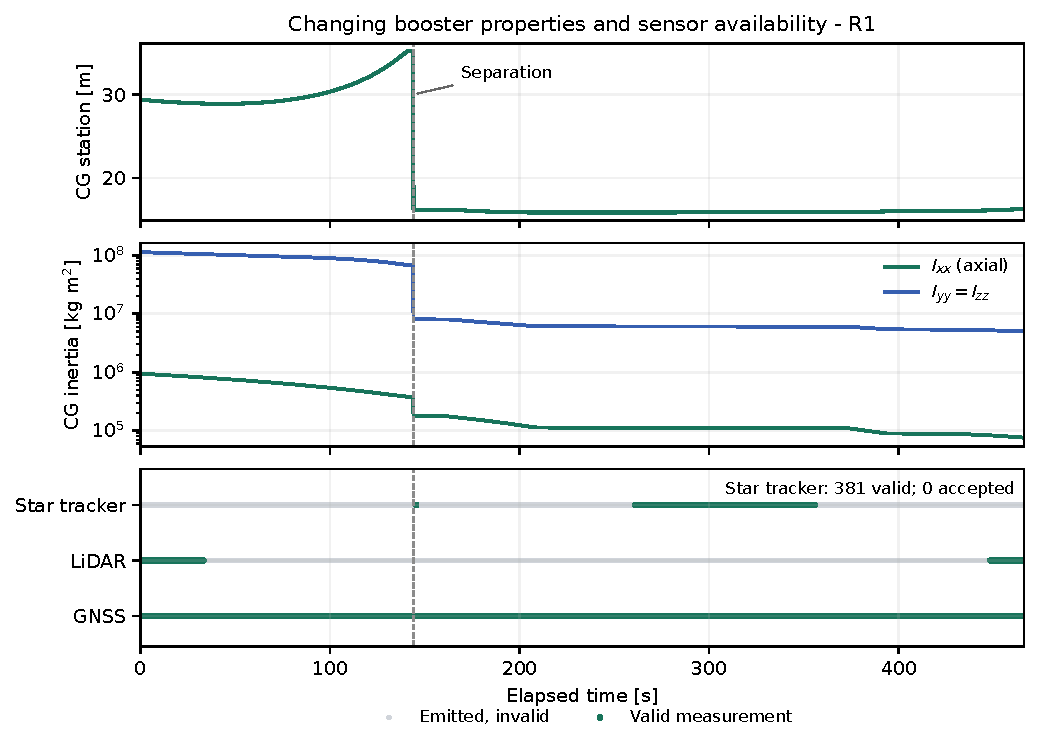
\includegraphics[width=.95\linewidth]{images/appendix_properties_availability.pdf}
\captionof{figure}{R1 properties and sensor validity. The dashed line marks separation at 144 s: the CG/inertia jump changes the tracked configuration, while structural-point states remain continuous. Green samples are valid and gray invalid. IMU validity is continuous and omitted from the panel. All 381 valid star exposures are accepted by the unchanged NIS gate.}
\label{fig:app-properties-availability}
\end{minipage}\par\smallskip

\noindent\begin{minipage}[t]{.45\linewidth}
\centering\small
\captionof{table}{R1 sensor counts. The first IMU sample primes history; 46508 subsequent samples propagate the filter. Other used samples correct it.}\label{tab:app-sensor-counts}
\setlength{\tabcolsep}{3pt}
\begin{tabular}{@{}lrrr@{}}
\toprule
Sensor & Emitted & Valid & Used \\
\midrule
IMU & 46509 & 46509 & 46509 \\
GNSS & 4651 & 4651 & 4651 \\
LiDAR & 4651 & 496 & 496 \\
Star & 1861 & 381 & 381 \\
\bottomrule
\end{tabular}
\end{minipage}\hfill
\begin{minipage}[t]{.51\linewidth}
\centering\small
\captionof{table}{Contact metrics under the two timing settings. Same target and acceptance limits.}\label{tab:app-variant}
\setlength{\tabcolsep}{3pt}
\begin{tabularx}{\linewidth}{@{}Xrr@{}}
\toprule
Metric & R1 & R2 \\
\midrule
Max. step [s] & 0.01 & 0.05 \\
IMU rate [Hz] & 100 & 20 \\
Contact time [s] & 465.0827 & 465.1900 \\
Vertical speed [m/s] & 0.4975 & 0.5030 \\
Horizontal speed [m/s] & 0.9016 & 0.7404 \\
Tilt [deg] & 0.5349 & 1.8062 \\
Angular rate [deg/s] & 0.01289 & 0.11308 \\
Target error [m] & 3.3061 & 6.1705 \\
Contact criteria & Pass & Pass \\
\bottomrule
\end{tabularx}
\end{minipage}\par
